%@descr: A template for a paper, a report or a thesis - suitable for modifications
%@author: Maciej Komosiński

\documentclass{article} 
\usepackage[english]{babel} 
\usepackage[utf8]{inputenc} 
\usepackage[T1]{fontenc}
\usepackage{graphicx} %include pdf's (and png's for raster graphics... avoid raster graphics!)
\usepackage{amsmath} %just for \eqref
\usepackage{url}
\usepackage{subcaption} % or \usepackage{subfigure}
\usepackage{float} % for [H] placement specifier
\usepackage{multicol}
\usepackage{microtype}
\usepackage[pdftex,hyperfootnotes=false,pdfborder={0 0 0}]{hyperref}
%\usepackage{caption_2019-09-01} % after all packages; pdfborder not implemented the same way for every implementation because the specification is imprecise; under miktex you just don't see the frames


% Changing the size of the text page
\addtolength{\voffset}{-2cm}
\addtolength{\hoffset}{-2cm}
\addtolength{\textwidth}{4cm}
\addtolength{\textheight}{4cm}

% More reasonable parameters controlling the placement of figures
\renewcommand{\topfraction}{.85}
\renewcommand{\bottomfraction}{.7}
\renewcommand{\textfraction}{.15}
\renewcommand{\floatpagefraction}{.66}
\renewcommand{\dbltopfraction}{.66}
\renewcommand{\dblfloatpagefraction}{.66}
\setcounter{topnumber}{9}
\setcounter{bottomnumber}{9}
\setcounter{totalnumber}{20}
\setcounter{dbltopnumber}{9}

% Custom bullet list with small vertical spacing
\newenvironment{tightlist}{
\begin{itemize}
  \setlength{\itemsep}{1pt}
  \setlength{\parskip}{0pt}
  \setlength{\parsep}{0pt}}
{\end{itemize}}

% We are looking for images in the following directory:
\graphicspath{{pics/}}



%\title{}
%\author{}
%\date{}


\begin{document}

\thispagestyle{empty} %no page number

\begin{center}
{\large{Machine Learning Theory:\\
Miniproject\\
}}

\vspace{3ex}

Computational experiment: Kolmogorov-Arnold Networks

\vspace{3ex}
{\footnotesize\today}

\end{center}


\vspace{10ex}

Lecturer: dr hab.~inż. Wojciech Kotłowski, prof. PP

\vspace{5ex}

Authors:
\begin{tabular}{lllr}
\textbf{Jędrzej Warczyński} & inf148234 & AI & jedrzej.warczynski@student.put.poznan.pl \\
\textbf{Mateusz Zwierzchowski} & inf148xxx & AI & mateusz.zwierzchowski@student.put.poznan.pl \\
\end{tabular}

\vspace{25ex}

\noindent We declare that this report and the accompanying source code has been prepared solely by the above author(s), and all contributions from other sources have been properly indicated and are cited in the bibliography.

\newpage






\begin{abstract}
Kolmogorov-Arnold Networks (KANs), proposed as a promising alternative to Multilayer Perceptrons (MLPs),
employ learnable activation functions on edges, represented as spline functions, inspired by the Kolmogorov-Arnold representation theorem.
This paper investigates the influence of spline order and grid size on training, validation, and test accuracy, as well as loss, in KAN networks.
Experimental analyses are conducted on two datasets, MNIST and CIFAR10, to explore the performance of KANs under varying parameters.
\end{abstract}

\section{Introduction}\label{sec:introduction}

KANs\cite{liu2024kan}, introduced as a promising alternative to Multilayer Perceptrons (MLPs),
are inspired by the Kolmogorov-Arnold representation theorem rather than the universal approximation theorem that underpins MLPs.
While MLPs utilize fixed activation functions on nodes, KANs employ learnable activation functions on edges, represented as spline functions.
This unique architecture eliminates traditional linear weight matrices in favor of a flexible and adaptive framework, potentially offering advantages in accuracy and parameter efficiency.

The focus of our research lies in understanding how spline order and grid size impact the training, validation, testing accuracy, and loss in KANs.
Through extensive empirical experiments conducted on two datasets, MNIST and CIFAR10, we aim to elucidate the optimal configuration of KANs for various tasks and datasets.

\section{Experiments}\label{sec:experiments}

\subsection{Experimental Setup}\label{subsec:experimental-setup}

We conduct experiments on the MNIST and CIFAR10 datasets to evaluate the performance of Kolmogorov-Arnold Networks (KANs) with varying spline orders and grid sizes.
The grid size is a critical parameter, dictating the number of control points for the spline functions that define the learnable activation functions on the network's edges.
It modulates the granularity of the spline approximation, allowing for finer or coarser representations of data.
Conversely, the spline order determines the degree of the spline polynomials used in these activation functions, influencing the complexity and flexibility of the model's response to input variations.
\newline
\newline
Our experimental setup includes:
\begin{itemize}
    \item Network Configuration: 4 layers with the number of nodes in the hidden layers set at 128, 64, 32, and 10, respectively.
    \item Optimization: We use the Adam optimizer with a learning rate of 0.001, exponential decay of 0.8, and a batch size of 64.
    \item Duration: The training process spans 10 epochs.
    \item Performance Metrics: We assess the KANs based on training, validation, and test accuracies, as well as loss metrics.
\end{itemize}

\noindent Specific training configurations tested include:
\begin{itemize}
    \item Models with a fixed spline order of 3 across various grid sizes (5, 10, 20, 40, 80, 160, 320, 640, and 1280).
    \item Models with a constant grid size of 5 and varying spline orders from 2 to 12.
\end{itemize}

\noindent To enhance visualization, all figures depicting training accuracy and loss are smoothed using a moving average with a window size of 2 and a scaling factor of 0.9.
\newline

\subsection{MNIST Dataset}\label{subsec:mnist}

The MNIST dataset consists of 60,000 training and 10,000 testing grayscale images of handwritten digits.

\subsubsection{Grid Size Influence}\label{subsubsec:grid-size-influence}

We present the comparison of training and validation loss in Figure~\ref{fig:mnist_loss_grid_size}
and the comparison of training, validation, and test accuracy in Figure~\ref{fig:mnist_accuracy_grid_size} for KANs with varying grid sizes.


\begin{figure}[H]
    \centering
    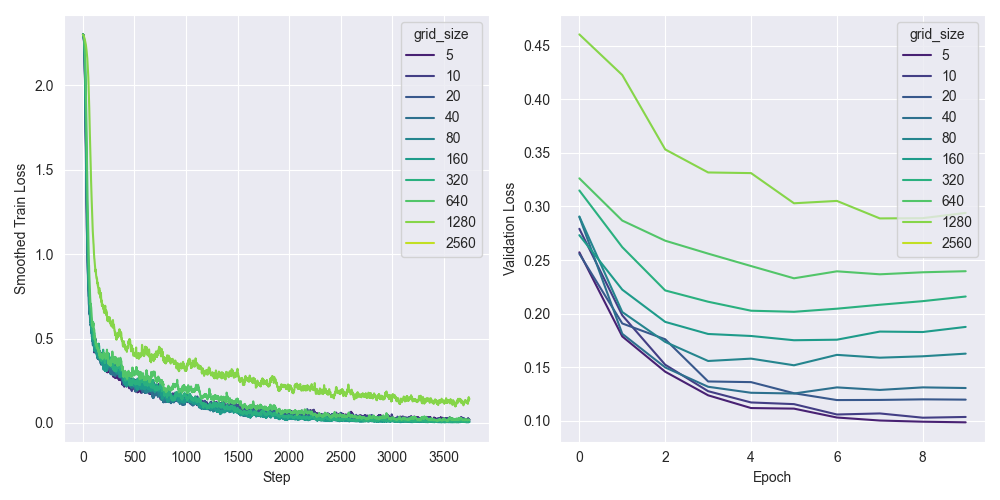
\includegraphics[width=0.9\textwidth]{pics/mnist_loss_grid_size}
    \caption{Training and validation loss comparison for MNIST.}
    \label{fig:mnist_loss_grid_size}
\end{figure}

\begin{figure}[H]
    \centering
    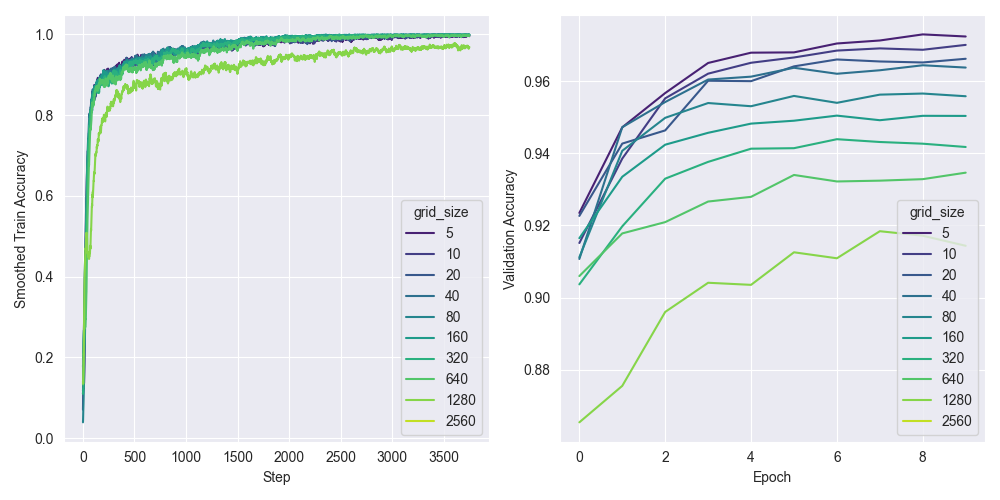
\includegraphics[width=0.9\textwidth]{pics/mnist_accuracy_grid_size}
    \caption{Training, validation, and test accuracy comparison for MNIST.}
    \label{fig:mnist_accuracy_grid_size}
\end{figure}


\subsubsection{Spline Order Influence}\label{subsubsec:spline-order-influence}

We present the comparison of training and validation loss in Figure~\ref{fig:mnist_loss_spline_order}
and the comparison of training, validation, and test accuracy in Figure~\ref{fig:mnist_accuracy_spline_order} for KANs with varying spline orders.

\begin{figure}[H]
    \centering
    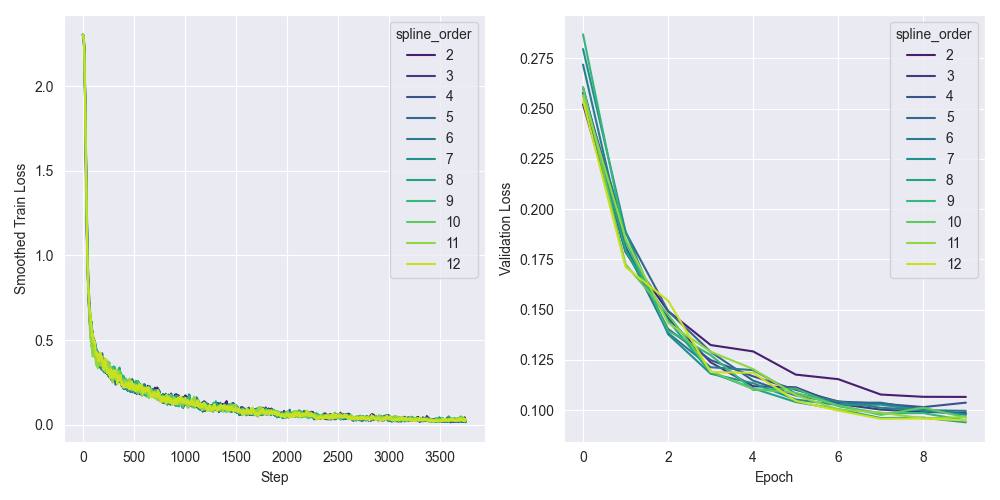
\includegraphics[width=0.9\textwidth]{pics/mnist_loss_spline_order}
    \caption{Training and validation loss comparison for MNIST with varying spline orders.}
    \label{fig:mnist_loss_spline_order}
\end{figure}

\begin{figure}[H]
    \centering
    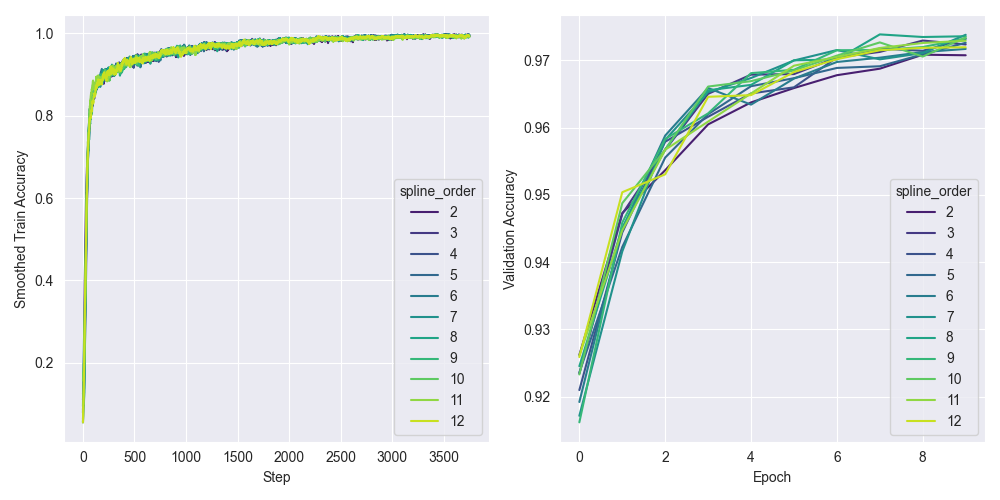
\includegraphics[width=0.9\textwidth]{pics/mnist_accuracy_spline_order}
    \caption{Training, validation, and test accuracy comparison for MNIST with varying spline orders.}
    \label{fig:mnist_accuracy_spline_order}
\end{figure}


\subsection{CIFAR10 Dataset}\label{subsec:cifar10}

The CIFAR10 dataset comprises 50,000 training and 10,000 testing color images of 10 classes.

\subsubsection{Grid Size Influence}\label{subsubsec:grid-size-influence-cifar10}

Similarly to the MNIST dataset, we present the comparison of training and validation loss in Figure~\ref{fig:cifar10_loss_grid_size}
and the comparison of training, validation, and test accuracy in Figure~\ref{fig:cifar10_accuracy_grid_size} for KANs with varying grid sizes.

\begin{figure}[H]
    \centering
    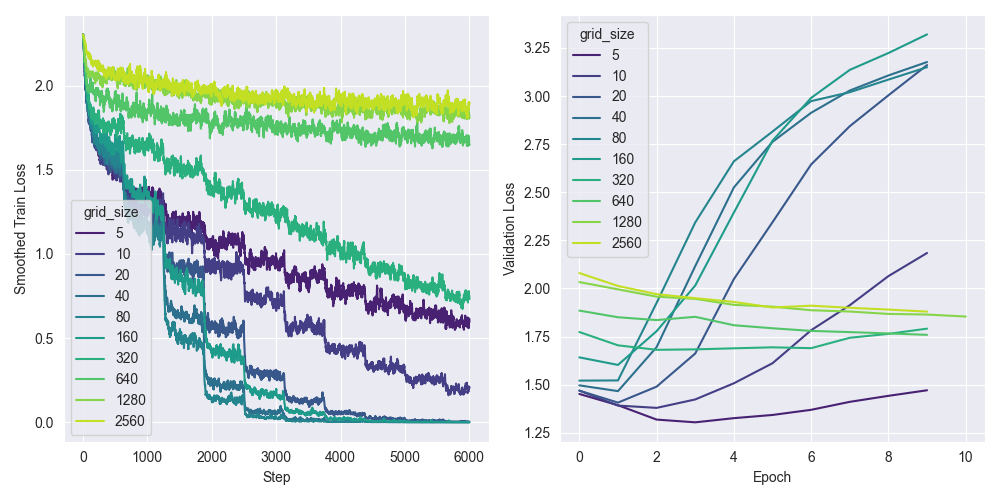
\includegraphics[width=0.9\textwidth]{pics/cifar10_loss_grid_size}
    \caption{Training and validation loss comparison for CIFAR10.}
    \label{fig:cifar10_loss_grid_size}
\end{figure}

\begin{figure}[H]
    \centering
    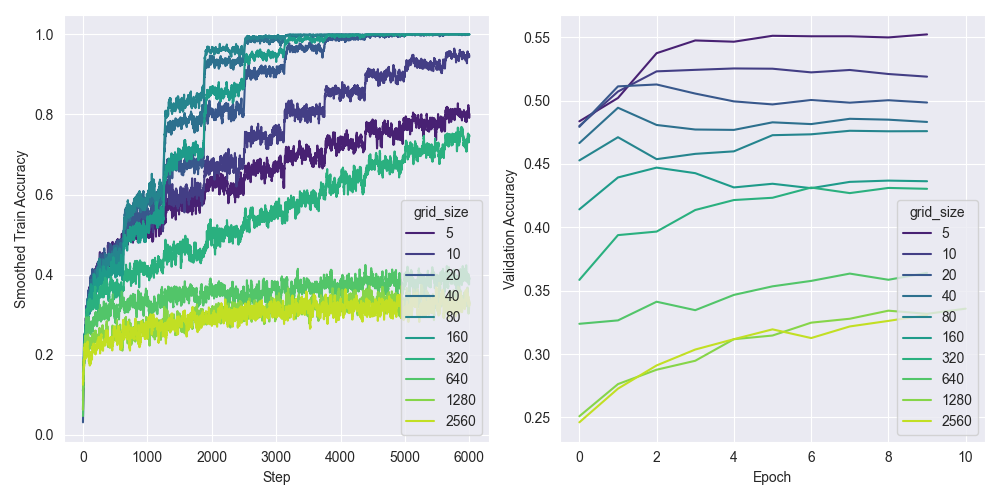
\includegraphics[width=0.9\textwidth]{pics/cifar10_accuracy_grid_size}
    \caption{Training, validation, and test accuracy comparison for CIFAR10.}
    \label{fig:cifar10_accuracy_grid_size}
\end{figure}


\subsubsection{Spline Order Influence}\label{subsubsec:spline-order-influence-cifar10}

Similarly to the MNIST dataset, we also present the comparison of training and validation loss in Figure~\ref{fig:cifar10_loss_spline_order}
and the comparison of training, validation, and test accuracy in Figure~\ref{fig:cifar10_accuracy_spline_order} for KANs with varying spline orders.

\begin{figure}[H]
    \centering
    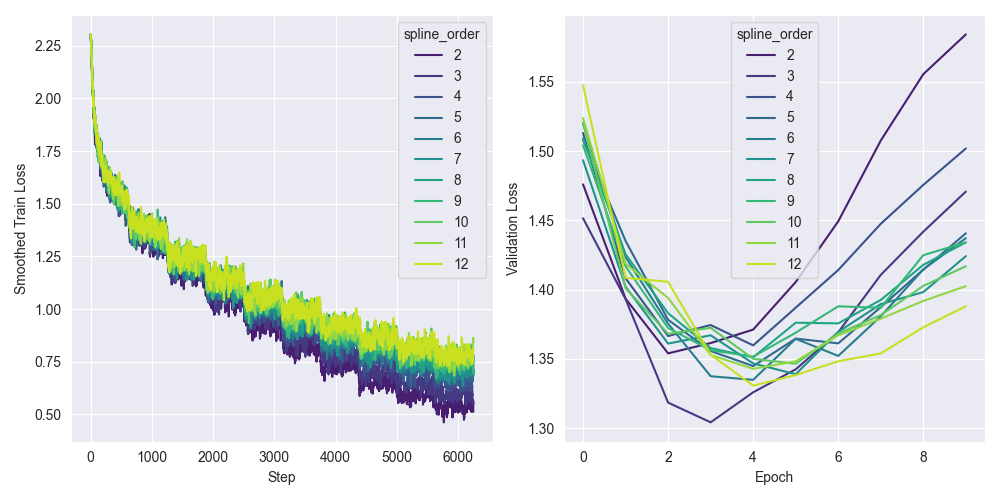
\includegraphics[width=0.9\textwidth]{pics/cifar10_loss_spline_order}
    \caption{Training and validation loss comparison for CIFAR10 with varying spline orders.}
    \label{fig:cifar10_loss_spline_order}
\end{figure}

\begin{figure}[H]
    \centering
    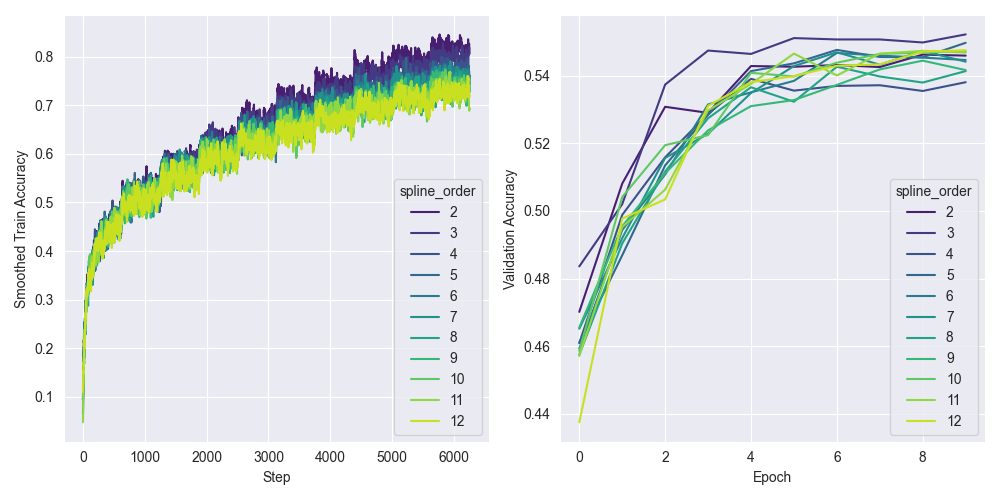
\includegraphics[width=0.9\textwidth]{pics/cifar10_accuracy_spline_order}
    \caption{Training, validation, and test accuracy comparison for CIFAR10 with varying spline orders.}
    \label{fig:cifar10_accuracy_spline_order}
\end{figure}


\section{Conclusions}\label{sec:conclusions}
Our experiments on Kolmogorov-Arnold Networks have elucidated the effects of grid size and spline order on model performance.
We found that larger grid sizes significantly enhance the model's capability to detail complex data patterns by providing more control points,
thereby allowing for finer adjustments to the activation functions.
This improvement in model granularity can markedly boost performance for tasks requiring detailed feature recognition.
However, it also raises the risk of overfitting and increases the computational burden.

Conversely, smaller grid sizes tend to simplify the model architecture,
which reduces computational demands and mitigates the risk of overfitting but may compromise the ability to capture complex patterns effectively.
In terms of spline orders, higher orders facilitate the capture of more intricate relationships within the data,
due to the increased complexity of the spline functions.
Although this complexity allows for a nuanced modeling of non-linear relationships, it simultaneously heightens the risk of overfitting and necessitates rigorous regularization strategies.
Lower spline orders produce simpler spline functions, which are less susceptible to overfitting and foster better generalization,
although they may overlook subtle intricacies in data features.

These observations highlight the critical balance between model complexity and performance efficacy,
underscoring the need for carefully selecting grid size and spline order based on the specific requirements and constraints of each task.
Looking ahead, the best approach would be developing adaptive mechanisms that can dynamically adjust these parameters in response to changes in data characteristics during training.
This approach could potentially optimize both the efficiency and accuracy of KANs across a broader range of applications.

\clearpage % let LaTeX put pending figures right here -- this command "releases" the accumulated content, which is useful if you have placed a lot of images, much more than text -- so they do not appear at the end of the document.


%%%%%%%%%%%%%%%% references %%%%%%%%%%%%%%%%

\bibliography{biblio}
\bibliographystyle{plain}


\end{document}
